\epstopdfsetup{outdir=./}
\section{Simulation Analysis}
\label{sec:simulation}

\subsection{Operating Point Analysis}

Table~\ref{tab:op_sim1} shows the simulated operating point results for the circuit
under analysis. Compared to the theoretical analysis results, one notices the
following differences: describe and explain the differences.

FALTA COLOCAR AS TABELAS DO NGSPICE

\begin{figure}[h] \centering
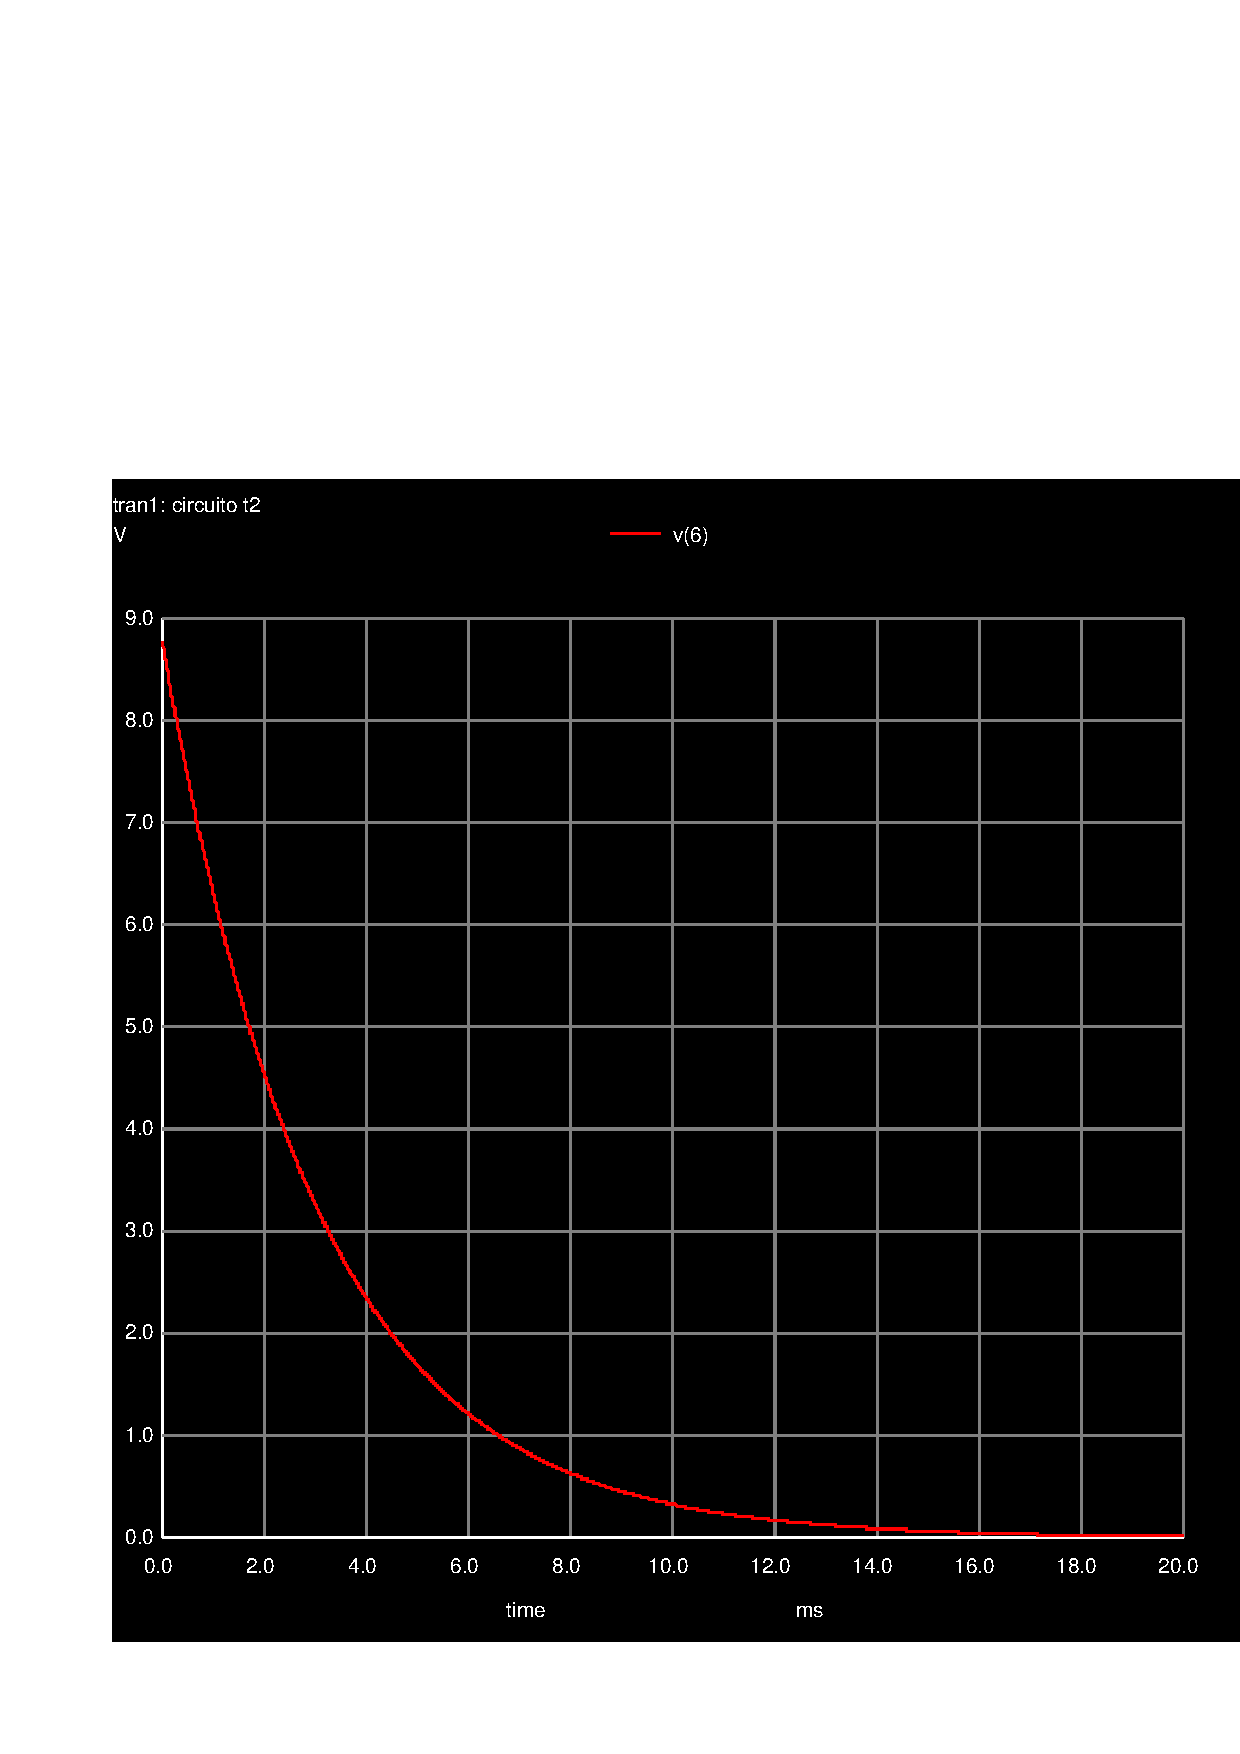
\includegraphics[width=0.6\linewidth]{trans.pdf}
\caption{Simulated natural response of $V_6(t)$ in the interval [0,20] ms. The \textit{x axis} represents the time in miliseconds and the \textit{y axis} the Potencial in node 6  in Volts.  }
\label{fig:sim_natural}
\end{figure}








